%%%%%%%%%%%%%%%%%%%%%%%%%%%%%%%%%%%%%%%%%%%%%%%%%%%%%
%% Inserir seu texto do referencial teorico no campo abaixo %%
%%%%%%%%%%%%%%%%%%%%%%%%%%%%%%%%%%%%%%%%%%%%%%%%%%%%%
\chapter{Referencial Teórico}
O referencial teórico do presente trabalho foi estruturado com base nos métodos tecnológicos utilizados na elaboração do projeto e alguns fatores que favorecem a escolha de tais métodos. Sendo estruturado em pequenos tópicos abordando cada uma das tecnologias, técnicas e linguagens de programação utilizadas na sua elaboração.
Essa etapa foi de suma importância, pois através dela foi obtido todo o fundamento primordial para elaboração e sustentação do projeto.


\section{Back-end}
Esta camada é responsável pela regra de negócio do \textit{software}, responsável ainda pela comunicação entre a base de dados e front-end, intermediando-as. O back-end tem a função de interagir com o banco de dados, solicitando/enviando informações, as quais são processadas e se obtém informações relevantes para o usuário. Diversas linguagens de programação podem ser utilizadas nesta camada, como: Kotlin, PHP, Java, Python, Go, etc.
\cite{universoprograma}

\subsection{Kotlin}
É uma linguagem estaticamente tipada desenvolvida pela JetBrains, cuja sintaxe é mais expressiva e concisa do que a do Java. Com recursos como expressões lambda, sobrecarga de operadores, templates de strings, suporte nativo a corotinas e outros.
Como Kotlin e Java são linguagens com alto grau de interoperabilidade, podem ser utilizadas juntas no mesmo projeto por serem executadas na mesma plataforma, a Java Virtual Machine (JVM).
A linguagem é utilizada de forma primária na implementação das camadas back-end e front-end \textit{mobile} no projeto.
\cite{kotlinemacao}

\subsection{GraphQL}
GraphQL é uma linguagem de requisições para API’s, que proporciona a seus usuários formulação de consultas exatamente como sua necessidade, tendo respostas em tempo de execução.
Foi criado em 2012 pelo Facebook, quando a empresa decidiu que precisava reconstruir seus aplicativos móveis nativos.
Enquanto as típicas API’s como REST utilizam vários carregamentos de URL’s, GraphQL obtém todos os dados em apenas uma única solicitação, trazendo somente os dados necessários. GraphQL proporciona que o desenvolvedor defina uma consulta aninhada e possa requisitar todos os dados em uma só busca.
Imagine uma rede social: Exibir uma publicação, exibir origens desta, pessoas que curtiram e as que comentaram, agruparem por pessoas que gostaram e que não gostaram da publicação. Isso seria muito custoso se realizado por REST por exemplo, pois para cada tipo de informação uma chamada seria realizada, enquanto em GraphQL, tudo isso pode ser obtido em uma única chamada, permitindo então que as aplicações fiquem mais rápidas, mesmo em conexões de redes móveis lentas.
GraphQL é baseado na computação distribuída, conceito amplamente difundido atualmente, onde aplicações são independentes de plataformas. Oferece solução para qualquer aplicação onde haja comunicação do tipo cliente-servidor via API, seja ela \textit{web}, \textit{desktop} ou \textit{mobile}, GraphQL pode ser utilizado.
Atualmente, essa tecnologia é um projeto de código aberto da GraphQL Foundation, hospedado pela Linux Foundation e mantido por várias empresas como: Airbnb, Apollo, Coursera, Facebook, GitHub entre outras.
Diversas empresas utilizam essa tecnologia, como: Audi, NBC, Atlassian, Twitter, Paypal e diversas outras.
\cite{graphqlrevolucionaria}


\section{Base de Dados}
Um SGBD é de extrema importância no gerenciamento e organização de dados, e o seu uso é indispensável, principalmente quando se trata de uma grande escala de dados. SGBD é uma coleção de programas que permitem a definição, construção e manipulação de dados, tais possibilidades são conhecidas respectivamente como: Linguagem de Definição de Dados (DDL), Linguagem de Controle de Dados (DCL) e Linguagem de Manipulação de Dados (DML).
Dado é tudo aquilo registrado como um fato que possa virar informação. Já a informação é o dado processado, de forma que possa ser relevante para uma organização. Em todas as fases, os dados ajudam às empresas nas tomadas de decisão, seja ela em nível operacional (tempo real) ou estratégico (tomada de decisão em longo prazo, quando o dado é transformado em informação), sendo assim, pode-se considerar que uma base de dados é o “coração” de uma empresa.
\cite{projetobdr}

\subsection{SQL Server}
O SQL Server (criado em 1998 pela Microsoft), é um SGBD relacional, onde os dados são estruturados de forma muito organizada, sendo então relacionados entre si, tendo maior persistência, melhor gerenciamento e confiabilidade, além de oferecer um ótimo desempenho pelo fato de distinguir os dados.
Sql Server é um dos principais SGBD`S relacionais e um dos mais utilizados pelas empresas atualmente, tendo como principal concorrente a Oracle.
Para qualquer empresa ou desenvolvedor que preze pelos seus dados é necessário que trabalhe com um SGBD que ofereça confiança e robustez.
Fez se então necessário que tal SGBD fosse escolhido, já que a aplicação irá trabalhar com dados de terceiros, sendo volumosos (necessidade de robustez) e de propriedade privada (o que requer segurança), sendo tais necessidades totalmente atendidas pelo SQL Server.
\cite{sqlserevralemdoconceito}


\section{Computação em nuvem}
Nos tempos atuais, é quase que imprescindível o uso da tão difundida computação em nuvem.
Esse tipo de computação oferece sob demanda poder computacional, armazenamento de banco de dados e toda a infraestrutura para uma aplicação de sucesso, tudo isso em rede, sendo usado como um hardware local. Tendo como vantagem o baixo custo por não ter que investir em hardwares próprios, economizando ainda por não ter manutenções.
Dentre diversas vantagens, é possível citar: maior segurança, melhor desempenho, melhor escalabilidade, extensibilidade, dentre outros.
\cite{computnuvem}

\subsection{Amazon Web Services}
A AWS, é uma empresa subsidiária da gigante Amazon, seu nicho de mercado é voltado para a computação em nuvem, fornecendo toda infraestrutura e componentes para sistemas distribuídos. Tem como ponto de destaque toda a facilidade oferecida em utilizar seus serviços, deixando os desenvolvedores a cargo somente da implementação do projeto. Outro fator positivo é a flexibilidade de seus planos, onde se tem a liberdade de adequá-los à escalabilidade do projeto, pagando somente o que usar.
Não é por acaso que ela é a maior empresa do nicho, sendo esta responsável por 47\% de toda a computação em nuvem do mundo. Como é mostrado na figura \ref{fig:awsnuvem}
\cite{aws2019}

\begin{figure}[H]
    \centering
        \caption{AWS no mercado de computação em nuvem.}
        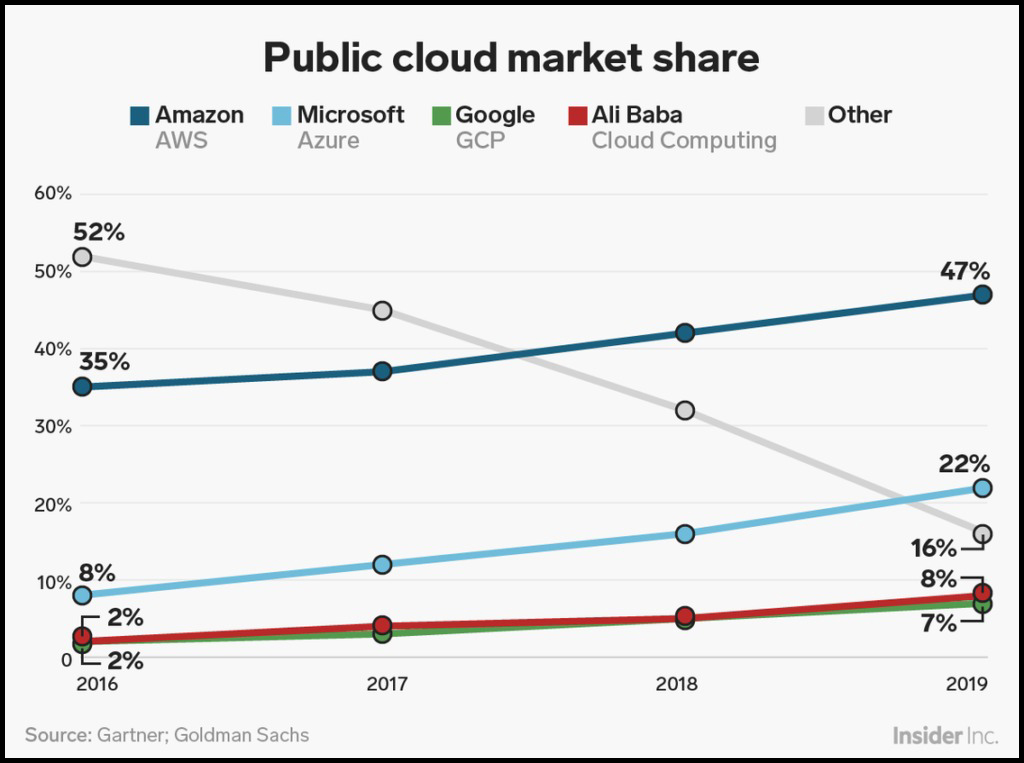
\includegraphics[scale=0.3]{Imagens/awsNomercadoCloud.jpg}
        \fonte{SERVICES(2019a)}
        \label{fig:awsnuvem}
\end{figure}

\subsubsection{Relational Database Service}
Um dos serviços oferecidos pela AWS é o RDS (Serviço de Base de dados relacionais), oferecendo poder de armazenamento sob demanda, evitando que desenvolvedores tenham que lidar com tarefas administrativas, podendo então concentrar-se somente no desenvolvimento. 
Com RDS é possível que o DBA coloque sua base de dados em zonas de disponibilidade, onde se cria o banco de dados em uma destas e habilita a função multi-AZ, fazendo com que o seu banco de dados fique replicado e sincronizado em tempo real, garantindo ainda mais segurança para seus dados e que este nunca pare, mesmo em caso de falha (caso ocorra a base de dados secundária assume exatamente onde a primeira estava).
O RDS da Amazon oferece vários tipos de instâncias de banco de dados, bem como oferece os principais mecanismos de bancos relacionais: SQL Server, Oracle Database, PostgreSQL, MariaDB, MySQL e até mesmo seu próprio mecanismo de banco de dados Amazon Aurora.
\cite{reladataservice}

\subsubsection{Elastic Beanstalk}
Outro serviço oferecido pela AWS é o Elastic Beanstalk, voltado para implantação de aplicações e serviços web desenvolvidos em Kotlin, .NET, PHP, Ruby, Go e Docker, em servidores mais utilizados como Apache, Nginx, Passenger e ISS. 
Assim como o RDS, o Elastic Beanstalk oferece diversas vantagens, como: escalabilidade, extensibilidade, toda a comodidade ao desenvolvedor, abstendo-o das atividades exaustiva de administração/configuração, propiciando que o mesmo só faça o \textit{upload} de seu código e o Elastic Beanstalk se encarregue de todo o gerenciamento da infraestrutura do servidor, como balanceamento de carga, redirecionamento http, conteiners e a execução do servidor propriamente dito, sendo seu maior atrativo o ganho de produtividade.
\cite{elasticbean}


\subsection{Google Cloud Platform}
A definição da própria Google sobre sua plataforma é: “O GCP consiste em um conjunto de ativos físicos, como computadores e unidades de disco rígido, e recursos virtuais, como máquinas virtuais (VMs), localizados nos centros de dados do Google em todo o mundo.” Em outras palavras alugamos parte do armazenamento de um \textit{Data Center} da Google, assim aproveitando uma infraestrutura de alta qualidade e extremamente segura pagando um valor simbólico.
Um fator que diferencia a hospedagem no Google Cloud é a sua rede toda feita com fibra óptica, que faz com que a perca de dados seja quase nula e com taxa de transferência extremamente alta. 
\cite{googlecp}

Segundo o \cite{googlecp} as principais vantagens são:
\begin{itemize}
\item Criação de aplicações de forma rápida;
\item Suportam Linux e Windows;
\item Boa base de conhecimento para solução de problemas.
\end{itemize}

\subsubsection{Application Programming Interface (API)}
API’s (Interface de Programação de Aplicações), são conjuntos de padrões/protocolos que permitem a construção e utilização de aplicativos de forma não tão evidente para usuários, onde sua solução ou serviço pode se comunicar com outros serviços sem precisar saber como eles foram implementados. Possibilitando assim, liberar o acesso aos seus recursos sem abrir mão da segurança e controle. Onde o desenvolvedor é quem define como isso será feito e quem terá acesso.
As API’s surgiram nos primórdios da computação, bem antes dos computadores domésticos, quando eram usadas como bibliotecas de sistemas operacionais.
O foco das API'S é simplificar a integração de novos componentes de aplicações a uma arquitetura já existente.
As API’s públicas acrescentam grande valor comercial porque simplificam e ampliam a forma como você se conecta aos parceiros, além de possivelmente monetizar seus dados. Um exemplo clássico é a API do Google Maps.
\cite{apiredhat}

\subsubsubsection{Routes}
Routes é uma API da Google Cloud voltada para mapas, sua função é disponibilizar o melhor trajeto entre dois pontos, levando em conta fatores como trânsito em tempo real.
É um serviço bastante completo, contendo 64 milhões de estradas catalogadas, 25 milhões de atualizações diárias e 1 bilhão de usuários ativos por mês, segundo informações da própria Google Cloud.
Tudo isso possibilita aos usuários ter o melhor trajeto entre origem e destino, podendo reduzir custos e tempo, seja por transporte coletivo ou privado.
Outro detalhe bastante interessante é o fato de exibir estimativas de trajetos em diversas formas de transportes, como de carro, ônibus/metrô, bicicleta e até mesmo a pé. 
Esta API possui três recursos essenciais:
Directions: Disponibiliza rota de transportes público ou privado, calculando o tempo de deslocamentos atuais ou futuros baseando-se no trânsito em tempo real.
Distance Matrix: Fornece distâncias de um ou mais trajetos e o tempo gasto neste.
Roads: Determina precisamente, o trajeto de um veículo.

As informações obtidas pela API dar-se por meio de interface HTTP, usando coordenadas de latitude e longitude para identificar os locais, acompanhando ainda sua chave de API. A plataforma de mapas do Google é paga, seu valor depende dos recursos integrados a ela, sendo levado em conta também o número de requisições de rotas ou distâncias. Entretanto, disponibilizam de forma gratuita um pacote de recursos com número relativamente alto de requisições, o que atendeu perfeitamente esse projeto.
\cite{routes}


\section{Engenharia de Software}
Embora a “crise do \textit{software}” tenha ocorrido em 1970, parece que esta nunca acaba, pois na atualidade muitos dos problemas enfrentados na época ainda rodeiam desenvolvimento de \textit{softwares}, desde projetos pequenos a sistemas super completos. Os problemas ainda assombram equipes de desenvolvimento, pois muitas das etapas e processos de engenharia de \textit{software} são negligenciados, seja por falta de interesse em produzir um bom \textit{software}, falta de verba para projeto, tempo mal gerenciado e etc.
A engenharia de software nasceu nos primórdios dos anos 70, durante “A crise do software”, onde projetos extrapolavam o prazos e orçamentos, \textit{softwares} possuíam baixíssimas qualidades e diversos problemas. Com o objetivo de saná-los, a engenharia de software surge com ferramentas, técnicas e processos sistematizados de se produzir software, os quais são aplicados nas fases de análise de projeto, documentação, desenvolvimento, validação, implantação, e evolução de software.
Dentre os diversos problemas que ainda persistem até então, pode se destacar:
Levantamento de requisitos mal feitos, onde equipes com a falsa sensação de produtividade já querem codificar de forma imediata, e para tal não absorvem as necessidades do cliente. Por outro lado, clientes omitem informações que, embora para ele seja óbvia mas para a equipe de desenvolvimento não.
Falta de comunicação entre cliente e desenvolvedor, esse problema ocorre dos dois pontos de vista, da visão de cliente, pensam que a equipe conhece totalmente suas necessidades, e muitos detalhes não são passados. Por outro lado, a equipe de desenvolvimento pode não ser muito detalhista quanto ao que é possível de se solucionar com softwares por exemplo.
Diversas organizações contratam gerentes de projetos com pouco \textit{know-how} ou ainda sem nenhum conhecimento de tecnologia. Estes muitas vezes possuem a falsa sensação de que ter equipamentos de modernos é o suficiente para sua equipe alcançar um \textit{software} de sucesso, ou ainda contratar mais programadores é a solução para o cronograma estourado.
Muitas empresas negligenciam por exemplo, a documentação de software, e no caso de contratação de nova equipe de desenvolvimento, torna se árduo sua manutenibilidade, já que a equipe não terá nenhuma base para conhecer o projeto. Fases de manutenção são ainda mais custosas que o desenvolvimento em si. \textit{Softwares} devem ser criados visando fácil manutenibilidade, atender requisitos de clientes, ter um bom padrão de qualidade, ser confiável e etc., pois o sucesso de uma empresa de desenvolvimento depende disso.
Para tal, técnicas de engenharia de software devem ser bem empregadas do início ao fim do projeto, ou ainda por toda sua existência, visando ter total controle do projeto. É possível que no futuro, as próprias tecnologias substituam programadores, mas nunca substituirá técnicas de engenharia de software.
\cite{engenhariadesoftware}


\section{Front-End}
O front-end é o cartão de visitas para uma aplicação, pois é neste que o usuário tem sua primeira impressão, antes mesmo de usá-la. Esta camada é crucial na comunicação/marketing da empresa pois no design deste, utiliza-se geralmente logotipos da empresa ou pelo menos padrões de cores relacionados a essa. Um front-end bem elaborado irá despertar nos usuários da aplicação, uma confiança de um software bem desenvolvido, e até mesmo definir o sucesso ou fracasso da aplicação.
\cite{universoprograma}

\subsection{Flutter}
Com a mesma proposta do React Native de criar aplicativos híbridos utilizando apenas uma base de código surgiu o Flutter em 2017, desenvolvido e atualizado pela equipe da Google, utilizando a linguagem Dart como base de criação dos aplicativos.
O Flutter fica na camada do UI e não chama os componentes nativos do SO, diferente do React Native que possui um intermediário entre a UI e o dispositivo. Trabalhando dessa forma traz uma performance muito mais rápida e fluida, e pode até mesmo ser comparada a um aplicativo feito de maneira nativa. Sua curva de aprendizado também é muito rápida e simples.
O Flutter trabalha com os "\textit{widgets}", que seria a mesma coisa de um componente. Um \textit{widget} é uma árvore que pode conter um ou mais filhos, e esses filhos são renderizados conforme a construção desta árvore. 
\cite{flutter}
A figura a seguir demonstra

\begin{figure}[H]
    \centering
        \caption{Um gráfico de radar mostrando a nota de 0–5 para cada critério em cada plataforma.}
        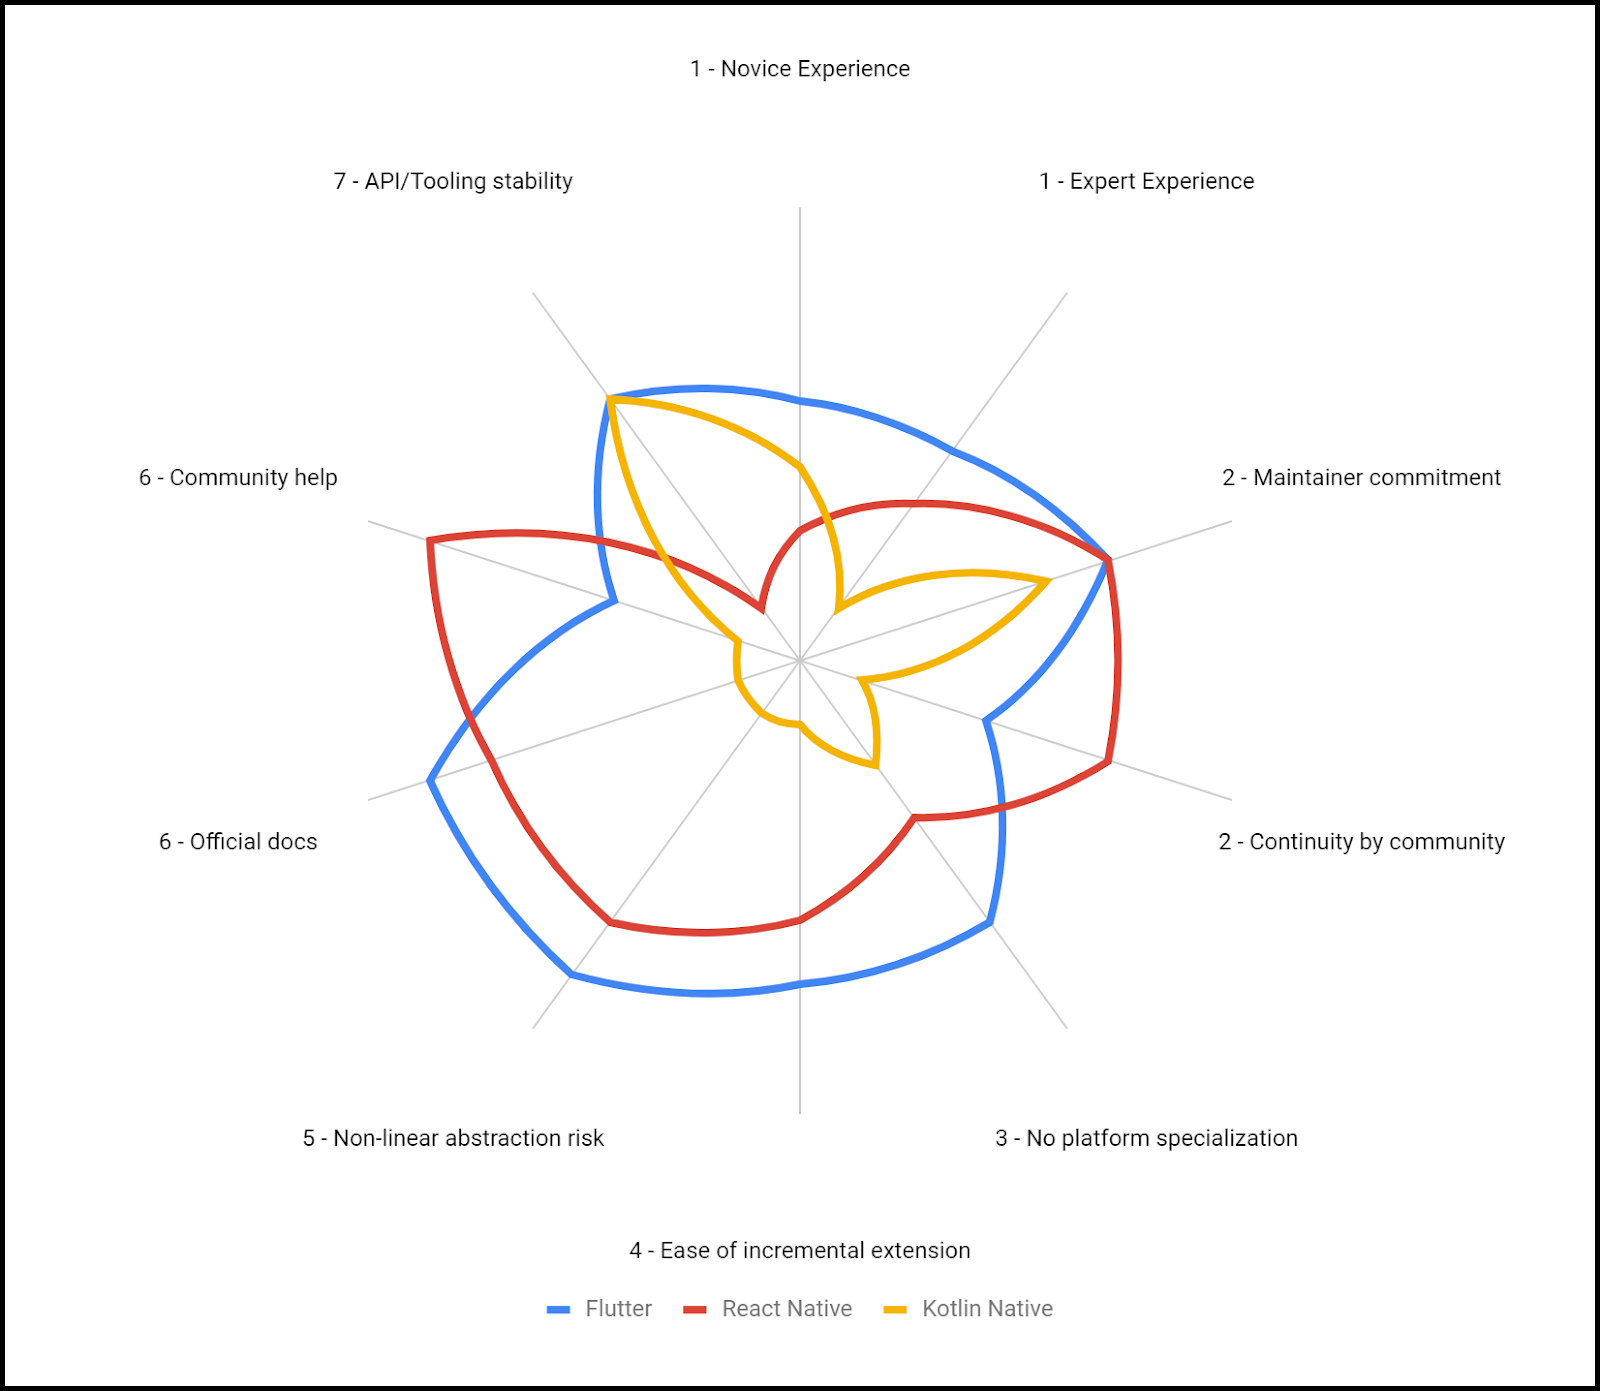
\includegraphics[scale=0.3]{Imagens/flutter.png}
        \fonte{(FREIRE,2019)}
        \label{fig:flutter}
\end{figure}


\section{Plataforma Mobile}
É indiscutível o uso de \textit{smartphone} atualmente, pois só no Brasil tem mais de um aparelho por pessoa, segundo a 29ª Pesquisa Anual de Administração e Uso de Tecnologia da Informação nas Empresas, realizada pela Fundação Getúlio Vargas de São Paulo (FGV-SP).

Sabendo disso, é notável a importância de se desenvolver para essa plataforma, além de outros fatores os quais aplicações \textit{mobile} se sobressaem entre as demais. Por exemplo, em uma aplicação \textit{web} tem se um tempo bem superior ao se conectar com um servidor, se comparado a um aplicativo mobile.
\cite{meirellespesquisa29}
